\chapter{The Perceptron}

In this chapter we will be going over the architecture of the most basic \keyword{neural network (NN)}, called the \keyword{perceptron}\sidenote{Also called Rosenblatt's perceptron}. 

\section{The Neuron}

The most basic unit of a perceptron is called the \keyword{neuron}\sidenote{More specifically, the McCulloch-Pitts model of a neuron}. The structure of a neuron can be seen in Figure \ref{neuron}, each neuron possesses the following.
\begin{bullets}
	\item Some \keyword{input features} $x_1\,\ldots\,x_n$
	\item A corresponding \keyword{weight} for each feature $w_1\,\ldots\,w_n$
	\item A \keyword{bias} $b$
	\item An \keyword{activation function} $\varphi(.)$
	\item An \keyword{output} $y$
\end{bullets}

\begin{marginfigure}\begin{tikzpicture}[>=Stealth, node distance=1.5cm, auto, myarrow]
	
	% Inputs
	\node[node, label=$x_1$, node distance=1cm] (inputa) {};
	\node[node, label=$x_2$, below of=inputa, node distance=1cm] (inputb) {};
	\node[label=$\vdots$, below of=inputb, node distance=1cm] (dots) {};
	\node[node, label=$x_n$, below of=dots, node distance=0.75cm] (inputc) {};
	
	% sum, bias and activation
	\node [node, right of = inputb] (sum) {};
	\node[node, above of = sum, label=$b$] (bias) {};
	\node[node, right of = sum, label=$\varphi(.)$] (activation) {};
	
	% output
	\node [node, right of = activation, label=$y$] (output) {};
	
	% connections
	\draw [myarrow, darkgray] (inputa) -- (sum) node[midway, above] {$w_1$};
	\draw [myarrow, darkgray] (inputb) -- (sum) node[midway, above] {$w_2$};
	\draw [myarrow, darkgray] (inputc) -- (sum) node[midway, above] {$w_n$};
	\draw [myarrow, darkgray] (bias) -- (sum); 
	\draw [myarrow, darkgray] (sum) -- (activation) node[midway, above] {$v$};
	\draw [myarrow, darkgray] (activation) -- (output);
	
\end{tikzpicture} \centering \caption{Signal Flow Graph of A Neuron} \label{neuron}  \end{marginfigure}

A neuron essentially performs the following operation, which can be seen from the signal flow graph.
\[ y = \varphi \left( \sum_{i=1}^{n} w_i x_i + b \right)\]

\section{The Basic Perceptron}

The perceptron was initially built with just a single neuron, and was limited to performing \keyword{binary classification} or \keyword{linear regression.}
\begin{bullets}
	\item In binary classification, each training sample $(X,y)$ contains some data $X=x_1 , x_2, \ldots$ and a label $y\in\left\{ -1, +1 \right\}$
	\item In linear regression the dependent variable is $y\in\mathbb{R}$
\end{bullets}
Overall, the perceptron was created to deal with binary classification problems.
\begin{bullets}
	\item This means that both classes $c_1$ and $c_2$ need to be \keyword{linearly seperable}\sidenote{We need to be able to draw a hyperplane that clearly seperates every instances from both classes, such that only instances from the same class are on a distinct side of the hyperplane}
	\item The perceptron is essentially trying to find a \keyword{linear separator} between the two classes\sidenote{Given that the activation function, $\varphi(.) \leftarrow \text{sgn}(.) $}, such that $\sum w_i x_i + b = 0$.
\end{bullets}

\section{Multi-Layered Perceptrons}

The most basic perceptron was basically a single-layered NN, but now we will discuss the \keyword{multi-layered perceptron (MLP)} which uses more layers, with possibly more neurons in each layer\sidenote{We do this to overcome the perceptrons practical limitations}.

Before I continue, lets clarify some terminology.
\begin{bullets}
	\item The \keyword{input layer} is the first layer with neurons that each accept 1 feature. In total, an input layer with $k$ neurons can accept $k$ features. 
	\item The \keyword{output layer} is the last layer, containing neurons that spit out one output each. In total an output layer with $h$ neurons produces an output with dimensionality of $h$.
	\item The \keyword{hidden layers} are the other layers sandwiched in between the input and output. When we say a "an $n$-layered network", we are referring to the amount of hidden layers in the network.
\end{bullets}
This is illustrated in Figure \ref{layers}.

\begin{marginfigure} \centering \caption{Layers in an MLP} \label{layers} 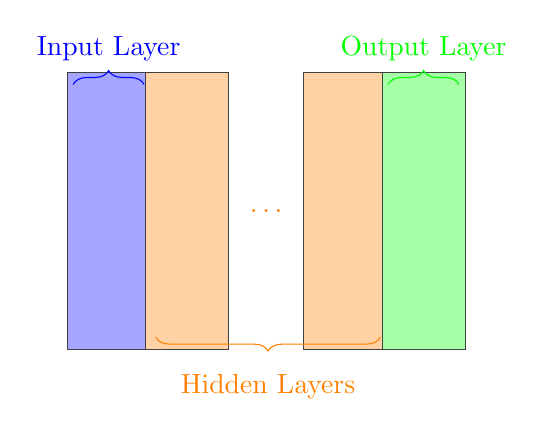
\begin{tikzpicture}[draw=darkgray]
	%diagram
	\node[draw, rectangle, minimum height=10em, minimum width=3em, fill=blue!35] (input) {};
	\node[draw, rectangle, minimum height=10em, right of = input, minimum width=3em, fill=orange!35] (hidden1) {};
	\node[right of = hidden1, text=orange] (dots) {$\ldots$};
	\node[draw, rectangle, minimum height=10em, right of = dots, minimum width=3em, fill=orange!35] (hidden2) {};
	\node[draw, rectangle, minimum height=10em, right of = hidden2, minimum width=3em, fill=green!35] (output) {};
	
	%labels
	\draw [blue,decorate, decoration={brace,amplitude=5pt, raise=4ex}] (-0.45,1) -- (0.45,1) node[midway, yshift=3em, text=blue] {Input Layer};
	\draw [green, text=green, decorate, decoration={brace,amplitude=5pt, raise=4ex}] (3.55,1)-- (4.45,1) node[midway, yshift=3em] {Output Layer};
	\draw [orange, text=orange, decorate, decoration={brace,amplitude=5pt, mirror, raise=4ex}] (0.6,-1) -- (3.45,-1) node[midway, yshift=-3.5em] {Hidden Layers};
\end{tikzpicture} \end{marginfigure}

In order to construct a MLP we must ensure the following.
\begin{bullets}
	\item The activation function $\varphi_i (.)$ of each neuron $i$ is a \keyword{differentiable} and non-linear function.
	\item The network contains at least one layer that is \keyword{hidden} from the input and output nodes (hidden layers).
	\item The network exhibits a high degree of \keyword{connectivity} through synaptic weights of the network.
\end{bullets}
These conditions ensure that the network becomes complex, but also so complex that we struggle to understand the behavior of the network.

\section{Batch \& Iterative Learning}

As we work our way up to understanding the training of the MLP we should account for the two methods of teaching the MLP, called \keyword{batch learning} and \keyword{iterative learning}\sidenote{In the textbook this is called \emph{on-line learning} but this was obviously confusing so I changed it for this note.}
\begin{bullets}
	\item Batch learning consists of presenting a batch of training examples to the network at the same time
	\item Iterative learning consists of presenting one training example to the network at a time.
\end{bullets}

Batch learning has the advantages of  providing an accurate-estimation of the gradient vector, and allowing a parallelization of the learning process. While iterative learning is simple to implement and can utilize redundancies in the dataset.
